%mac
\begin{vidu}%book%SBT KNTT 19.3
Gọi tên các lực sau:
\begin{center}
\begin{tabular}{|l|c|}
\hline \textbf{Đối tượng} & \textbf{Tên gọi} \\
\hline \begin{tabular}{l} 
Lực do chất lỏng tác dụng lên một vật \\
nằm trong lòng chất lỏng đứng yên.
\end{tabular} &...............................\\
\hline Lực làm mòn hai bề mặt tiếp xúc nhau. & ............................... \\
\hline \begin{tabular}{l}
Lực tác dụng lên một quả táo chín\\ rời cành làm nó rơi xuống đất. \end{tabular} & ............................... \\
\hline Lực giữ bạn đứng yên trên sàn nhà. &............................... \\
\hline \begin{tabular}{l}
Lực giữ quả cầu treo dưới một sợi\\ dây khi cân bằng. \end{tabular} &............................... \\
\hline \begin{tabular}{l} 
Lực được tạo ra do sự chênh lệch áp suất\\ 
giữa hai bề mặt ở phía trên và phía dưới\\ cánh máy bay khi máy bay đang bay
\end{tabular} &............................... \\
\hline
\end{tabular}
\end{center}
\loigiai{
\begin{center}
\begin{tabular}{|c|c|}
\hline 
\textbf{Đối tượng}	& \textbf{Tên gọi} \\ 
\hline 
Lực do chất lỏng tác dụng lên một vật\\ 
nằm trong lòng chất lỏng đứng yên.&  Lực đẩy Archimedes.\\ 
\hline 
Lực làm mòn hai bề mặt tiếp xúc nhau.	&  Lực ma sát.\\ 
\hline 
Lực tác dụng lên một quả táo chín rời cành làm nó rơi xuống đất.	& Trọng lực. \\ 
\hline 
Lực giữ bạn đứng yên trên sàn nhà.	&  Phản lực.\\ 
\hline 
Lực giữ quả cầu treo dưới một sợi dây khi cân bằng.	&  Lực căng.\\ 
\hline 
Lực được tạo ra do sự chênh lệch áp suất giữa \\
hai bề mặt ở phía trên và phía dưới cánh máy bay khi máy bay đang bay	&  Lực nâng.\\ 
\hline 
\end{tabular}
\end{center}
}
\haidong{10} \end{vidu}
\begin{vidu}%SBT CTST 12.1
\immini[thm]{Hình bên biểu diễn các lực tác dụng lên quả tennis có khối lượng $56\ g$ đang rơi thẳng đứng. Coi lực nâng của không khí là không đáng kể. Hãy cho biết $\vec D$ là lực gì. Gia tốc của quả tennis có độ lớn là bao nhiêu $m/s^2$ (làm tròn kết quả đến chữ số hàng đơn vị)?
}{\begin{tikzpicture}
\node[] at (0,0){
\includegraphics[width=1cm]{images/tennis}};
\draw[->,very thick,red](0,0)--++(90:1)node[right,black]{$\vec{D}\ (0,2\ N)$};
\draw[->,very thick,blue](0,0)--++(-90:3)node[right,black]{$m\vec{g}\ (1\ N)$};
\draw[fill=white](0,0)circle(1.3pt);
\draw[->,very thick](-1,1)--++(-90:2)node[below,black]{Chiều (+)};
\end{tikzpicture}}
\shortans[oly]{14}	
\haidong{6}\loigiai{
\begin{itemize}
\item Lực $\vec D$ là lực cản của không khí.
\item Theo định luật 2 Newton, gia tốc của vật có độ lớn: $a=\dfrac{mg-D}{m}\approx 14\ m/s^2$, có hướng theo chiều dương chuyển động.
\end{itemize}
}
\haidong{10} \end{vidu}
\begin{vidu}%SBT KNTT III.8
Một người nhảy dù có khối lượng tổng cộng $100\ kg$. Trong thời gian đầu (khoảng vài giây) kể từ khi bắt đầu nhảy xuống, người này chưa mở dù và rơi dưới tác dụng của trọng lực. Khi người đó mở dù, lực tác dụng của dù lên người là $2000\ N$, hướng lên. Lấy $g=10\ m/s^2$.	
\begin{enumerate}[label=\alph*)]
\item Xác định hợp lực tác dụng lên người nhảy dù khi mở dù.
\item Người sẽ chuyển động như thế nào ngay sau khi mở dù?
\end{enumerate}
\haidong{10}\loigiai{
\begin{itemize}
\item[a)] Hợp lực tác dụng lên người nhảy dù hướng lên và có độ lớn $F=1000\ N$.
\item[b)] Khi chưa mở dù, người nhảy dù chuyển động nhanh dần đều dưới tác dụng của trọng lực (rơi tự do). 
\item Ngay sau khi mở dù, người nhảy dù sẽ chuyển động chậm dần đều với gia tốc: $a=-\dfrac{F}{m}=-\dfrac{1000}{100}=-10\ m/s^2$.
\end{itemize}
}
\haidong{10} \end{vidu}
\begin{vidu}%SBT KNTT III.9
\immini[thm]{
Con tàu trong hình bên đang chuyển động theo một hướng xác định với vận tốc không đổi.
\begin{itemize}
\item[a)] Xác định lực đẩy $\vec F_1$ của nước.
\item[b)] Xác định lực cản $\vec F_3$ của nước.
\end{itemize}
}{\begin{tikzpicture}
\node[] at (0,0){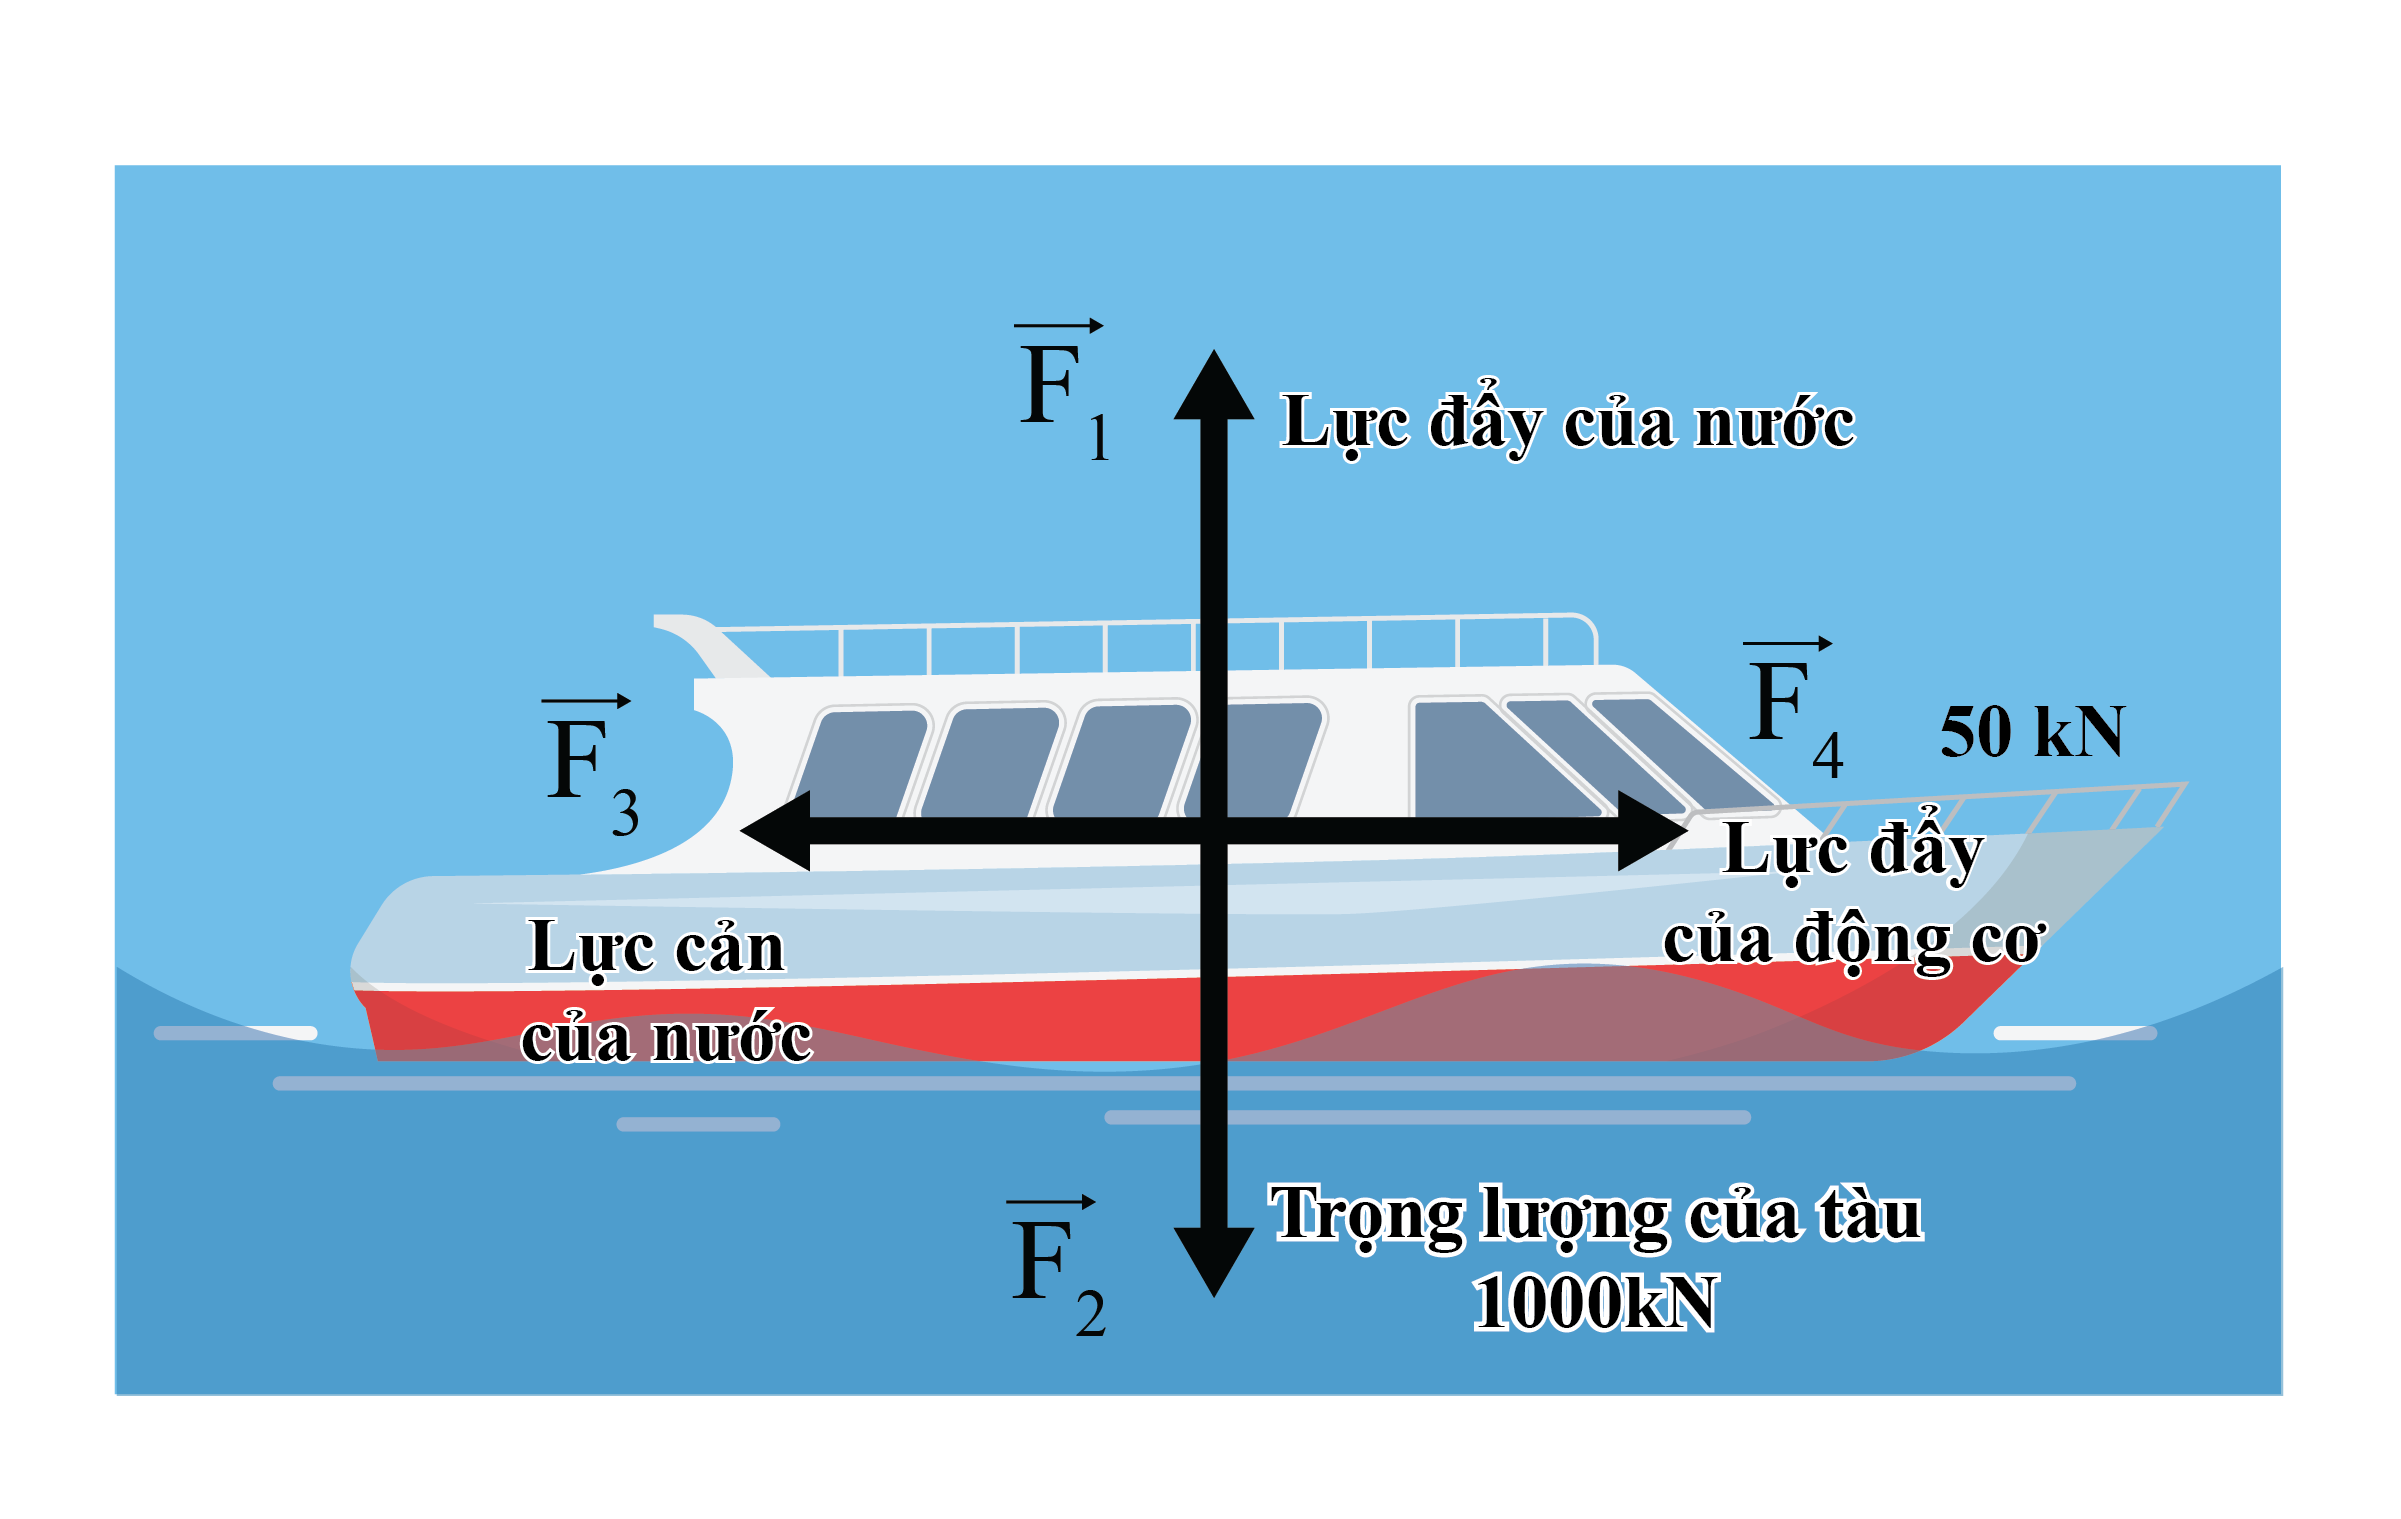
\includegraphics[width=5cm]{Images/2262}};
\end{tikzpicture}}	
\haidong{6}\loigiai{
\begin{itemize}
\item[a)] Vì con tàu chuyển động theo hướng xác định với vận tốc không đổi nên gia tốc của tàu là $a=0$.
\item Do đó tàu ở trạng thái cân bằng và hợp lực tác dụng $F=0$. 
\item[b)] $F_1=1000\ kN$.
\item[c)] $F_3=50\ kN$.
\end{itemize}
}
\haidong{10} \end{vidu}
\begin{vidu}%SBT CTST 11.9
Một vật làm bằng sắt và một vật làm bằng hợp kim có cùng khối lượng được nhúng vào cùng một chất lỏng. Hỏi lực đẩy Archimedes tác dụng lên vật nào lớn hơn và lập tỉ số giữa hai lực đẩy Archimedes này? Biết trọng lượng riêng của sắt và hợp kim lần lượt là $787,4\ N/m^3$ và $675,0\ N/m^3$.
\haidong{16}\loigiai{
\begin{itemize}
\item Theo giả thiết: $m_s=m_{hk}\Rightarrow \dfrac{V_s}{V_{hk}}=\dfrac{\rho_{hk}}{\rho_s}=\dfrac{6750}{7874}=0,857$
\item Ta có: $\dfrac{\left(F_A\right)_s}{\left(F_A\right)_{hk}}=\dfrac{\rho_{cl}.g.V_s}{\rho_{cl}.g.V_{hk}}=\dfrac{V_s}{V_{hk}}=0,857$
\item Vật lực đẩy Archimedes tác dụng lên vật làm bằng hợp kim lớn hơn lực đẩy Archimedes tác dụng lên vật làm bằng sắt 1,17 lần.
\end{itemize}
}
\haidong{10} \end{vidu}	
\begin{vidu}%SBT CTST 12.4
\immini[thm]{Một hòn đá được thả rơi vào chất lỏng. Sau một khoảng thời gian, người ta quan sát thấy hòn đá chuyển động thẳng đều. Khi đó, các lực tác dụng lên vật được biểu diễn như hình bên. Hình bên đã biểu diễn đủ các lực tác dụng lên vật chưa? Nếu chưa, hay bổ sung và tính độ lớn của lực còn thiếu.}{\begin{tikzpicture}[draw=Mapcolor]
\shade[ball color=Mapcolor] (0,0) circle (1.3ex);
\draw[->,very thick,red](0,0)--++(90:1)node[right,black]{$\vec{F}_A\ (0,5\ N)$};
\draw[->,very thick,blue](0,0)--++(-90:2.5)node[right,black]{$m\vec{g}\ (2,5\ N)$};
\draw[fill=white](0,0)circle(1.3pt);
\end{tikzpicture}}
\haidong{5}\loigiai{
\begin{itemize}
\item Hình 12.3 còn thiếu lực cản của nước.
\item Khi hòn đá chuyển động thẳng đều: $F_c=P-F_A=2,5-0,5=2\ N$.
\end{itemize}	
}
\haidong{10} \end{vidu}	








\begin{vidu}
Một chiếc xe máy đang chuyển động trên mặt đường ngang, tổng khối lượng người và xe là $200\ kg$. Lực đẩy do động cơ tác dụng lên xe máy là $500\ N$, tổng lực cản và ma sát lên xe máy là $50\ N$. Gia tốc xe máy có độ lớn là
\choice
{$1,25\ m/s^2$}
{\True $2,25\ m/s^2$}
{$3,25\ m/s^2$}
{$4,25\ m/s^2$}
\haidong{6}
\loigiai{
Chọn B

Chọn chiều dương là chiều chuyển động của ô tô

Gia tốc ô tô:

$
F=F_{\text {dây}}-F_{\text {cản}}=500-50=8=450\ N
$

$
a=\dfrac{F}{m}=\dfrac{450}{200}=2,25\left(\dfrac{m}{s^2}\right)
$

}
\haidong{10} \end{vidu}


\begin{vidu}
Một vật bằng kim loại chìm trong bình chứa nước thì nước trong bình dâng lên $100\ cm^3$. Cho khối lượng riêng của nước là $1000 \ kg/m^3$. Lấy $g=10\ m/s^2$. Lực đẩy của nước tác dụng lên vật là
\choice
{$4\ N$}
{$2\ N$}
{\True $1\ N$}
{$3\ N$}
\haidong{2}
\loigiai{
Chọn B
Lực đẩy của nước: $F=\rho \cdot g \cdot V=1\ N$

}
\haidong{10} \end{vidu}

\begin{vidu}%SBT CTST 11.8
Một vật có trọng lượng riêng $22.10^3\ N/m^3$. Lấy trọng lượng riêng của nước là $10^4\ N/m^3$. Treo vật vào một lực kế rồi nhúng vật ngập trong nước thì lực kế chỉ $30\ N$. Nếu treo vật ở ngoài không khí thì lực kế chỉ
\choice
{$40\ N$}
{$45\ N$}
{$50\ N$}
{\True $55\ N$}
\haidong{6}\loigiai{
\begin{itemize}
\item Khi nhúng vật vào trong nước thì vật chịu thêm lực Archimedes nên số chỉ của lực kế giảm xuống. Số chỉ của lực kế khi để ngoài không khí chính là trọng lượng của vật.
\item Khi vật cân bằng trong nước: $P-F_A=F\Rightarrow P-\dfrac{d_n}{d_v}.P=F$
\item Do đó, ta có: $P=\dfrac{F}{1-\dfrac{f_n}{d_v}}=55\ N$.
\end{itemize}
}
\haidong{10} \end{vidu}


\begin{vidu}%book%SBT CTST 10.7
\immini[thm]{Một vật chuyển động trong không khí, trong nước hoặc trong chất lỏng nói chúng đều sẽ chịu tác dụng của lực cản. Xét một viên bi thép có khối lượng $1\ g$ đang ở trạng thái nghỉ được thả rơi trong dầu. Người ta khảo sát chuyển động của viên bi trong dầu và vẽ đồ thị tốc độ theo thời gian của viên bi như hình. Cho biết lực đẩy Archimedes có độ lớn là $F_A=1,2.10^{-3}\ N$ và lấy $g=9,8\ m/s^2$. Độ lớn lực cản của dầu tác dụng lên viên bi sau thời điểm $t_2$ là bao nhiêu mili niutơn? 
}
{\begin{tikzpicture}[draw=Mapcolor]
\draw[->](0,0)--++(90:2.5)node[right]{$v\ (m/s)$};
\draw[->](0,0)--++(0:4.5)node[above]{$t\ (s)$};
\draw[dashed](0,2)--(4.5,2)(4,2)--(4,0)node[below]{$t_2$}(0.5,0.5)--(0.5,0)node[below]{$t_1$};
\draw[Mapcolor,very thick](0,0) to [bend left =27](4,2);
\end{tikzpicture}}
\shortans[oly]{8,6}
\haidong{6}\loigiai{
\begin{itemize}
\item Gọi $F_c$ (N) là độ lớn lực cản do dầu tác dụng lên viên bi,
\item Dựa vào đồ thị, ta thấy kể từ thời điểm $t_2$ trở về sau thì viên bi sẽ chuyển động thẳng đều.
\item Chọn chiều dương thẳng đứng hướng xuống, ta có: $P=F_A+F_c$.
\item Suy ra $F_c=P-F_A=8,6.10^{-3}\ N$
\end{itemize}
}
\haidong{15} \end{vidu}
